%!TEX program = Xelatex
\documentclass{article}
%\usepackage{ctex}
\usepackage{amsmath,amscd,amsbsy,amssymb,latexsym,url,bm,amsthm}
\usepackage{epsfig,graphicx,subfigure}
\usepackage{enumitem,balance,mathtools}
\usepackage{wrapfig}
\usepackage{mathrsfs, euscript}
\usepackage[usenames]{xcolor}
\usepackage{hyperref}
\usepackage{caption}
%\usepackage{subcaption}
\usepackage{float}
\usepackage{listings}
%\usepackage{enumerate}
%\usepackage{algorithm}
%\usepackage{algorithmic}
%\usepackage[vlined,ruled,commentsnumbered,linesnumbered]{algorithm2e}
\usepackage{algorithm}  
\usepackage{algorithmicx}  
\usepackage{algpseudocode}


\newtheorem{theorem}{Theorem}[section]
\newtheorem{lemma}[theorem]{Lemma}
\newtheorem{proposition}[theorem]{Proposition}
\newtheorem{corollary}[theorem]{Corollary}
\newtheorem{exercise}{Exercise}[section]
\newtheorem*{solution}{Solution}

\renewcommand{\thefootnote}{\fnsymbol{footnote}}

\newcommand{\postscript}[2]
    {\setlength{\epsfxsize}{#2\hsize}
    \centerline{\epsfbox{#1}}}

\renewcommand{\baselinestretch}{1.0}

\setlength{\oddsidemargin}{-0.365in}
\setlength{\evensidemargin}{-0.365in}
\setlength{\topmargin}{-0.3in}
\setlength{\headheight}{0in}
\setlength{\headsep}{0in}
\setlength{\textheight}{10.1in}
\setlength{\textwidth}{7in}

\title{CS222 Homework 6}
\author{Algorithm Analysis \& Deadline: 2020-10-20 Firday 24:00}
\date{Exercises for Algorithm Design and Analysis by Li Jiang, 2020 Autumn Semester}

\begin{document}

\maketitle

\begin{enumerate}

\item An adventure game uses a graph $G$ consisting of $N$ rooms (numbered from $1$ to $N$) to represent the places need to be explored. These rooms can only be linked in one-way, meaning that a person passing through this path can only move from one room to another but cannot return to the room they left/explored. It’s worth noting that there is no circle in this graph. People taking part in the game appear randomly in any of the rooms connected via corridors, and we can explore rooms in the same corridor. You should note that the path taken by two players may contain some of the same rooms.

How many players are the minimum needed to explore all the rooms?

Describe your design first and write down your algorithm in the form of pseudo-code.

~\\
\textbf{Solution.}\\~\\
\textbf{Problem Def.} Given a DAG, find the least paths to cover all the vertices. (Paths can overlap).\\~\\
We note the vertices set as $V$, and the edges set as $E$. To limit the visit times of vertices, we split every vertice $v$ into 2 vertices $v_i, v_o$ and add an directed edge $(v_i, v_o)$ with capacity $[1,+\infty)$. For every $e=(u,v)\in E$, replace it with a new edge $(u_o, v_i)$ with capacity $[0,+\infty)$. Add two new vertices $st$, $en$, and for every $v_i$ add an new edge $(st, v_i)$ with capacity $[0,1]$ representing whether a player starts at $v$, and for every $v_o$ add an new edge $(v_o, en)$ with capacity $[0, \infty]$ because more than 1 players can finish at $v$. \\
~\\
\begin{figure}[htb]
    \centering
    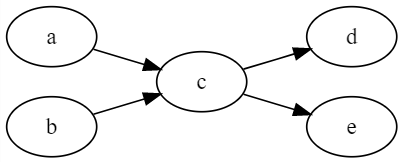
\includegraphics[width=0.4\textwidth]{1.png}
    \caption{origin graph}
    \label{fig1}
\end{figure}
\begin{figure}[htb]
    \centering
    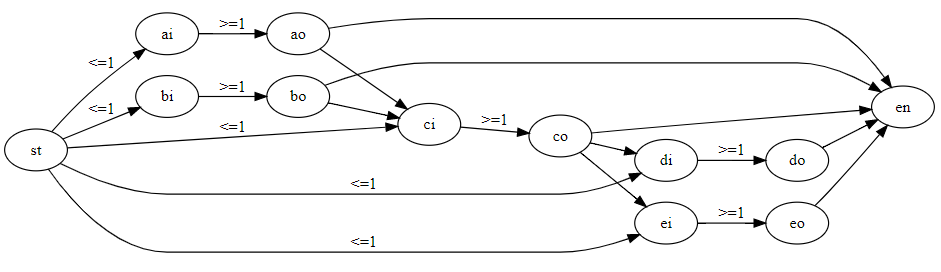
\includegraphics[width=0.8\textwidth]{2.png}
    \caption{graph for network}
    \label{fig2}
\end{figure}
\noindent We have constructed a new graph $G'$ with capacity. Figure \ref{fig1}, \ref{fig2} shows an example. We need to find the minimum flow statisfying these capacity limits. For this problem, 
I have two ideas:  
\begin{itemize}
\item [(1)] Binary search the answer.\\
Set a demand $d_v$ for every vertice $v$, $d_v = \sum_{e\ in\ v} f_e - \sum_{e\ out\ v} f_e$. Initially, $d_v = 0$ for all $v$, except $d_{st} = -c, d_{en} = c$, where $c$ is the answer we need to check. For all $e=(u,v)$ with capacity $[1,+\infty)$, remove the lower bound limit by $d_u\leftarrow d_u + 1, d_v\leftarrow d_v - 1$. And then add a source $s$ and a sink $t$, and for every $v$ with $d_v<0$ add an edge $(s, v)$ with capacity $|d_v|$, and for every $v$ with $d_v>0$ add an edge $(v, t)$ with capacity $|d_v|$. 
\\
Then run a $s\rightarrow t$ max flow on the network. If all the edge out of $s$ has a full flow i.e. $f_e = c_e$, then $c$ players are enough; otherwise $c$ players are not enough. We can find the minimum number of players by binary searching $c$. \textbf{Time complexity:} $O(nm\log n)$ (because the flow is at most $n$ and a $BFS$ process is $O(m)$).
\item[(2)] Find the minimum flow straightly.\\
The network structure is almost the same as the one above, but we set $d_{st}=d_{en}=0$ this time. Instead, we add an additional edge $(en, st)$ with capacity $[0, +\infty)$. We run a $s\rightarrow t$ max flow on this network to check whether there exists a circulation statisfying the demand limits. Then we get a feasible flow. And next, we remove the vertice $s$ and $t$ (and all edges linked to $s$, $t$), and remove the edge $(en, st)$. And then we run a $en\rightarrow st$ max flow on this network. Now, $\sum_{e\ out\ st} f_e$ is the minimum number of players needed.
Briefly proof:\begin{itemize}
    \item After running $s\rightarrow t$ max flow, we get a feasible circulation.
    \item After running $en\rightarrow st$ max flow, the circulation is still feasible, because we remove all the edge associated with demand $d_v$ and this process only sends back the redundancy.
    \item The second process sends back the redundancy as much as possible, so the remain is minimum.  
\end{itemize}
\end{itemize}
Algorithm \ref{algP1} shows the pseudo-code for idea (1).\\
\begin{minipage}[H]{0.9\textwidth}
\begin{algorithm}[H]
\caption{Pseudo Code for Problem 1}
\label{algP1}
\begin{algorithmic}[1]
    \Require{$G=(V,E)$}
    \Ensure{$num$ the number of minimum players needed}
    \Function{FindTheLeastPlayers}{$G=(V,E)$}
        \State $V'\leftarrow \emptyset, E'\leftarrow\emptyset$
        \State $V'\leftarrow V'\cup \{st, en, s, t\}$
        \For {$v \in V$}
            \State $V' \leftarrow V'\cup \{v_i, v_o\}$ // split vertice and add edge
            \State $E' \leftarrow E'\cup \{(v_i, v_o, c=\infty)\}$
            \State $E' \leftarrow E'\cup \{(st, v_i, c=1), (v_o, en, c=\infty)\}$
            \State $E' \leftarrow E'\cup \{(vi, t, c=1), (s, v_o, c=1)\}$ // deal with demand
        \EndFor
        \State $L\leftarrow 1, R\leftarrow |V|$
        \While{$L \leq R$}
            \State $C = \lfloor(L + R) / 2\rfloor$
            \State $G' = (V', E'\cup\{(s, st, c=C), (en, t, c=C)\})$
            \State$flow\leftarrow 0$
            \While {\Call{FindAugmentPath}{$G'$, $s$, $t$}}
                \State $flow \leftarrow flow +$\Call{Augment}{$G'$, $s$, $t$}
            \EndWhile
            \If {$flow$ == $|V|+C$} // means all the demands are satisfied, hence the circulation is valid
                \State $R\leftarrow C-1$ // $[C, R]$ is valid, then search in $[L, C-1]$
            \Else 
                \State $L\leftarrow C+1$ // $[L, C]$ is invalid, then search in $[C+1, R]$
            \EndIf
        \EndWhile
        \If {$L \leq |V|$}
            \State \Return {$L$}
        \Else
            \State throw No Feasible Solution Error
        \EndIf
    \EndFunction
\end{algorithmic}
\end{algorithm}
\end{minipage}\\~\\
And Algorithm \ref{dinic} shows the pseudo code of max flow algorithm (Dinic) here.\\
\begin{minipage}[htb]{0.9\textwidth}
\begin{algorithm}[H]
\caption{Dinic algorithm}
\label{dinic}
\begin{algorithmic}[1]
    \Function{findAugmentedPath}{$G=(V,E)$, $s$, $t$}
    \State $Q\leftarrow$ an empty queue, and add $s$ into $Q$, and mark $s$ as visited.
    \While{$Q$ is not empty}
        \State Take out the head $u$ of $Q$.
        \For {$e=(u, v)$ out of $u$}
            \If {$c_e > 0$ \textbf{and} $v$ is not visited}
                \State Set the precursor of $v$ as $u$.
                \If {$v == t$} 
                    \State \Return {True}
                \EndIf
                \State Add $v$ into $Q$, and mark $v$ as visited.
            \EndIf
        \EndFor
    \EndWhile
    \State \Return {False}
\EndFunction
\State
\Function{Augment}{$G=(V,E)$, $s$, $t$}
    \State $flow \leftarrow +\infty$
    \State $path \leftarrow $ an empty stack
    \While {$t$ != $s$}
        \State $u\leftarrow$ the precursor of $t$
        \State $flow = \min\{flow, c_{(u,t)}\}$
        \State Add edge $(u, t)$ into $path$
        \State $t\leftarrow u$
    \EndWhile
    \For {edge $e$ in $path$}
        \State $c_e \leftarrow c_e - flow$
        \State $c_{re} \leftarrow c_{re} + flow$ // re means the residual edge of $e$. 
    \EndFor
    \State \Return {flow}
\EndFunction
\end{algorithmic}
\end{algorithm}
\end{minipage}
~\\
\item Suppose there are $M \times N$ rooms, each of which holds a different number of treasures. Please select several rooms so that the selected rooms have no common sides (i.e., the selected rooms cannot be adjacent), and the selected rooms' treasures add up to the greatest value.
Describe your design first and write down your algorithm in the form of pseudo-code.

Note: The value of the treasure is definitely not negative.


~\\
\textbf{Solution.}\\
\begin{itemize}
    \item [1.] Define $V_1 = \{room: (x,y)|x + y \equiv 1 \mod 2\}$, $V_0=\{room:(x,y)|x+y\equiv 0 \mod 2\}$.
    \item [2.] For every room $u\in V_0$, if another room $v$ is adjacent to $u$, then add an directed edge $(u,v)$ with capacity $+\infty$. We claim that we has constructed a bipartite graph $G=(V=V_0\cup V_1,E=\{(u,v)|u\in V_0\wedge u,v\ are\ adjacent\})$, because two rooms $u, v$ are adjacent if and only if $(u
\in V_0\wedge v\in V_1) \vee (u\in V_1 \wedge v\in V_0)$.
    \item [3.] And then we add a source $s$ and a sink $t$, and for every $u\in V_0$ add an edge $(s, u)$ with capacity equal to $u$'s treasure, and for every $v\in V_1$ add an edge $(v, t)$ with capacity equal to $v$'s treasure. And we define that $(s,u)$ having flow means we select room $u$, and $(v,t)$ having flow means we select room $v$.
    \item [4.] If we select two adjacent rooms, we say that there is a contradiction. We assert that there is a contradiction if and only if there is a flow from the source $s$ to the sink $t$. Briefly proof: \begin{itemize}
            \item [$\Rightarrow$] A contradiction $\Rightarrow$ we select two adjacent room $u\in V_0, v\in V_1$ $\Rightarrow$ a flow $s\rightarrow u \rightarrow v \rightarrow t$
            \item [$\Leftarrow$]  A flow $s\rightarrow u\rightarrow v\rightarrow t$ $\Rightarrow$ we select $u\in V_0, v\in V_1$, and $u,v$ are adjacent $\Rightarrow$ a contradiction. 
            \end{itemize}
    \item [5.] We need to give up as minimum as possible treasure $(s,u), (v,t)$ to make the network disconnected, i.e. we need to work out the \textbf{minimum cut}. And $max\ treasure = total\ treasure - minimum\ cut = total\ treasure - max\ flow$.
\end{itemize}
\begin{figure}[htb]
\centering
\begin{minipage}[H]{0.25\linewidth}
    \centering
    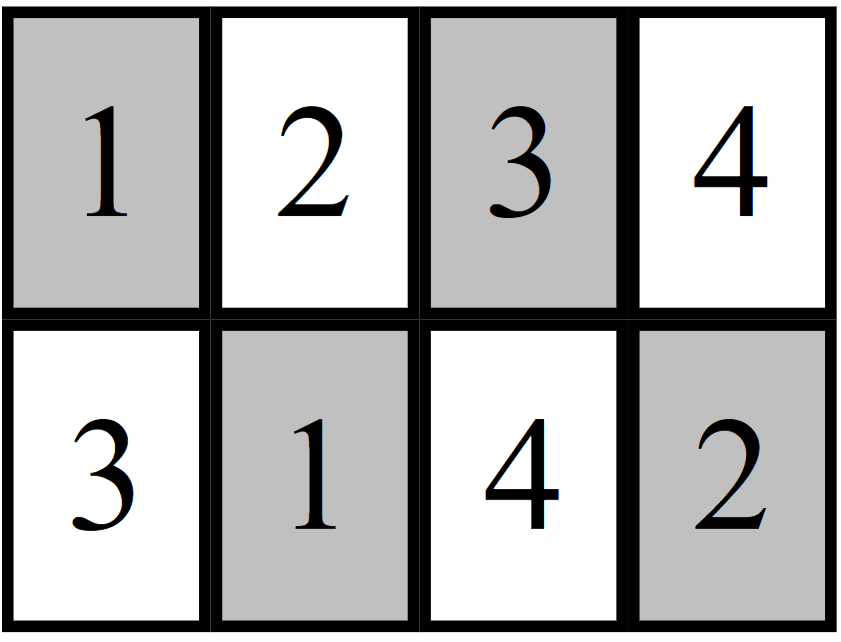
\includegraphics[width=1.0\linewidth]{3.png}
    \caption{An example for P2}
    \label{fig3}
\end{minipage}
\begin{minipage}[H]{0.5\linewidth}
    \centering
    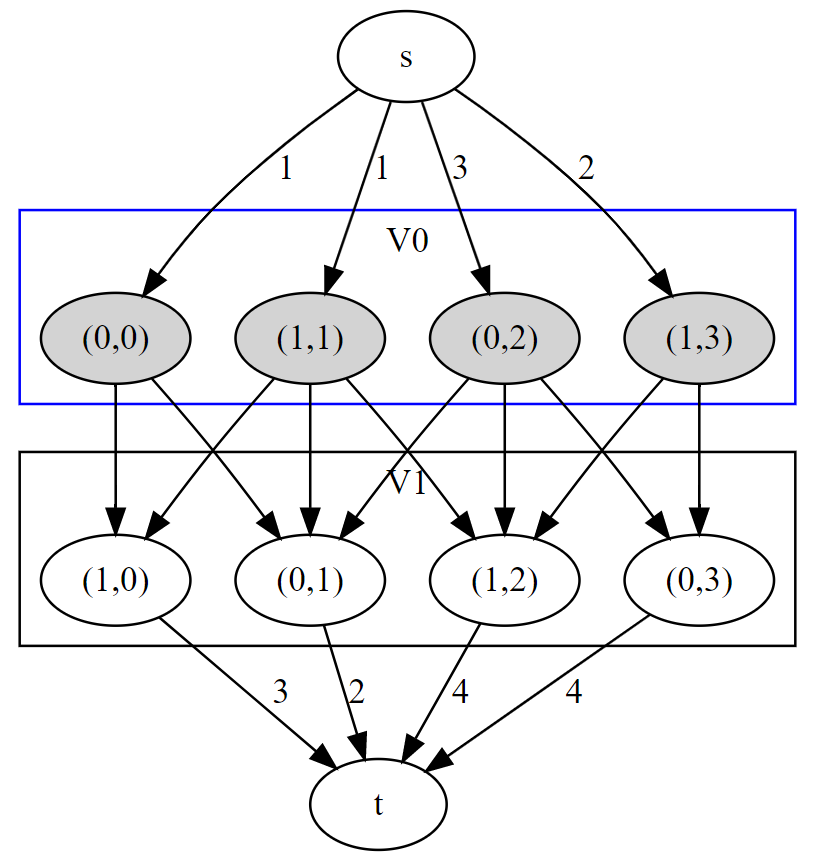
\includegraphics[width=1.0\linewidth]{4.png}
    \caption{Network for Figure \ref{fig3}}
    \label{fig4}
\end{minipage}
\end{figure}
Figure \ref{fig3} shows an example for this problem and Figure \ref{fig4} shows an network model constructed for the example.
\begin{minipage}[htb]{0.9\textwidth}
\begin{algorithm}[H]
\caption{pseudocode for P2}
\label{selectroom}
\begin{algorithmic}[1]
    \Require{An $M\times N$ grid $grid$ representing treasures in the rooms.}
    \Ensure{An set $selection$ representing selected rooms.}

    \Function{selectRooms}{$grid$}
        \State $E\leftarrow \emptyset$, $V\leftarrow \{rooms\ in\ $grid$\} \cup \{s, t\}$.
        \For {$room = (i,j)$ in $grid$}
            \If {$i+j \equiv 0 \mod 2$}
                \For {$room0 = (i0,j0)$ adjacent to $room=(i,j)$}
                    \State $E \leftarrow E\cup \{(room, room0, capacity=+\infty)\}$
                \EndFor
                \State $E \leftarrow E\cup \{(s, room, capacity=room.treasure)\}$
            \Else
                \State $E \leftarrow E\cup \{(room, t, capacity=room.treasure)\}$
            \EndIf
        \EndFor
        \State $G \leftarrow (V, E)$
        \While{\Call{findAugmentedPath}{$G, s, t$}}
            \State \Call{Augment}{$G, s, t$}
        \EndWhile
        \State $selection\leftarrow \emptyset$
        \For {$e=(s, room)\ or\ (room, t)$}
            \If {$c_e > 0$}
                \State $selection\leftarrow selection\cup\{room\}$ // \textit{remained capacity > 0 $\Rightarrow$ not in the min cut}
            \EndIf
        \EndFor
        \State \Return{$selection$}
    \EndFunction
\end{algorithmic}
\end{algorithm}
\end{minipage}
~\\~\\Algorithm \ref{selectroom} shows the pseudocode for Problem2, and the Dinic algorithm used here are showed in Algorithm \ref{dinic}.

~\\
\item There are a large number of servers in the data center. Each server has different performance, the program is executed on different servers with different efficiency, and now there is a set of the new programs that need to run. Please assign these programs to the appropriate server based on the historical test results to make this batch of programs run most efficiently. 
Describe your design first and write down your algorithm in the form of pseudo-code.

~\\
\textbf{Solution.}~\\
\textbf{Problem Def.} Given some programs $P=\{p_1,p_2,\cdots,p_n\}$ and some servers $Q=\{q_1,q_2,\cdots,q_m\}$, and a weight matrix $score_{n\times m}$. Find a match $(i, m_i)$ to maximize $score = \sum_{1\leq i\leq n} score_{i,m_i}$. If $n\ne m$ there may be some programs not being run or some servers not runing program.\\
We constructed a weighted bipartite graph:
\begin{itemize}
    \item A vertice set $V_0$ representing programs and a vertice set $V_1$ representing servers.
    \item For program $p_i$ and server $q_j$, add an directed edge $(p_i,q_j)$ with weight (or called cost) $MaxScore - score_{i,j}$, where $MaxScore:=\max{score_{i,j}} + 1$.
    \item If $|P| < |Q|$, we add $|Q|-|P|$ pseudo programs. For each pseudo program $p_i$ and each server $q_j$ add an directed edge $(p_i, q_j)$ with weight $MaxScore$.
    \item If $|Q| < |P|$, we add $|P|-|Q|$ pseudo servers. For each pseudo server $q_i$ and each program $p_j$, add an directed edge $(p_j, q_i)$ with weight $MaxScore$. 
\end{itemize}
Then we need to find a perfect match with minimum weight (or called cost).
Use the algorithm we talked in class. The correctness is proved in class, and hence I do not explain here. The pseudocode is showed in Algorithm \ref{P3}.\\
\begin{minipage}[htb]{0.9\textwidth}
\begin{algorithm}[H]
\caption{pseudocode for P3}
\label{P3}
\begin{algorithmic}[1]
    \Require{Program set $P=\{p_1,p_2,\cdots,p_n\}$, server set $Q=\{q_1,q_2,\cdots,q_m\}$ and score matrix $score_{n\times m}$}
    \Ensure{$Assignment$ = $\{(p_i,q_{match_i})|p_i\in P\}$}
    \Function{assignServer}{$P$, $Q$, $score$}
        \State $V\leftarrow P \cup Q \cup \{s, t\}$, $E\leftarrow \emptyset$, $Assignment \leftarrow \emptyset$, $MaxScore\leftarrow \max score_{i,j} + 1$
        \For{each $(p_i, q_j)$}
            \State $E \leftarrow E\cup \{(p_i, q_j, cost = MaxScore - score_{i,j})\}$
        \EndFor
        \If{$|P|<|Q|$}
            \For{$i \leftarrow |P|+1$ to $|Q|$}
                \State $V\leftarrow V\cup\{p_i\}$
                \For{each $q_j$}
                    \State $E\leftarrow E\cup\{(p_i, q_j, cost = MaxScore)\}$
                \EndFor
            \EndFor
        \EndIf
        \If{$|Q|<|P|$}
            \For{$i \leftarrow |Q|+1$ to $|P|$}
                \State $V\leftarrow V\cup\{q_i\}$
                \For{each $p_j$}
                    \State $E\leftarrow E\cup\{(p_j, q_i, cost = MaxScore)\}$
                \EndFor
            \EndFor
        \EndIf
        \State \textbf{foreach} $v\in V\setminus\{s,t\}$: $p(v)\leftarrow 0$
        \While{$Assignment$ is not a perfect matching}
            \State $dis\leftarrow$ shortest distances using costs $c^p(x,y) = p(x) + cost(x,y) - p(y)$
            \State $path\leftarrow$ shortest alternating path from $s$ to $t$ according to $dis$
            \State Update $Assignment$ after augmenting along $path$.
            \State \textbf{foreach} $v\in V\setminus\{s,t\}$: $p(v)\leftarrow p(v) + dis(v)$. 
        \EndWhile
        \State \Return {$Assignment$}
    \EndFunction
\end{algorithmic}
\end{algorithm}
\end{minipage}
~\\


\item Given a weighted directed graph $G(V, E)$ and its corresponding weight matrix $W=(w_{ij})_{n \times n}$ and shortest path matrix $D=(d_{ij})_{n \times n}$, where $w_{ij}$ is the weight of edge $(v_i, v_j)$ and $d_{ij}$ is the weight of a shortest path from pairwise vertex $v_i$ to $v_j$. Now, assume the weight of a particular edge $(v_a, v_b)$ is decreased from $w_{ab}$ to $w'_{ab}$. Design an algorithm to update matrix $D$ with respect to this change, whose time complexity should be no larger than $O(n^2)$. Describe your design first and write down your algorithm in the form of pseudo-code.
~\\~\\
\textbf{Solution.}~\\
I assume $w_{ij}\geq0, w'_{ab}\geq0$.\\
Consider the change of $d_{ij}$ after decreasing $w_{ab}$ to $w'_{ab}$: I think that $d'_{ij}=\min \{d_{ij}, d_{ia}+w'_{ab}+d_{bj}\}$ holds. Briefly proof: A new shortest path from $i$ to $j$ either passes by or does not pass by the directed edge $(a,b)$. If not passing by, $d'_{ij}=d_{ij}$ because other edges do not change. If passing by, $d'_{ij} = d'_{ia} + w'_{ab} + d'_{bj} = d_{ia} + w'_{ab} + d_{bj}$, because the shortest path from $i$ to $a$ and the shortest path from $b$ to $j$ do not pass by $(a,b)$ (assuming positive weight).
~\\
\begin{minipage}[htb]{0.9\textwidth}
\begin{algorithm}[H]
\caption{pseudocode for P4}
\label{P4}
\begin{algorithmic}[1]
    \Require{$W$,$D$,$a$,$b$,$w'_{ab}$}
    \Ensure{$D'=(d'_{ij})_{n\times n}$}
    \Function{UpdateDistance}{$W,D,a,b,w'_{ab}$}
        \For {$(i,j)\in \{1,2,\cdots,n\}\times\{1,2,\cdots,n\}$}
            \State $d'_{ij}=\min\{d_{ij}, d_{ia}+w'_{ab}+d_{bj}\}$
        \EndFor
        \State \Return{$D'=(d'_{ij})_{n\times n}$}
    \EndFunction
\end{algorithmic}
\end{algorithm}
\end{minipage}
~\\
Algorithm \ref{P4} shows my pseudocode for this problem, \textbf{Time complexity:} $O(n^2)$.
\item  Please review the papers to find an algorithmic problem related to the non-obvious network flow or circulation problem, summarize its problem formulation, and transform it into the network flow problem.
    
~\\
\textbf{Answer.}~\\
I reviewed the paper \textit{\href{https://doi.org/10.1145/2463209.2488824}{On effective and efficient in-field TSV repair for stacked 3D ICs. (DAC '13)}}, which was mentioned briefly in class. This paper describes a reconfigurable in-field repair solution to tolerate latent TSV (through-silicon-via) defects through the judicious use of spares.\\ 
~\\Problem formulation: Given a set of signals $S=\{s_1,s_2,\cdots,s_n\}$ and a set of TSVs $T=\{TSV_1,TSV_2,\cdots,TSV_m\}$, ($n<m$). The goal is to link every signal in $S$ with a dedicated TSV in $T$. Considering the physical constraints and design requirements of the actual problem, some links $(s, TSV)$ are invalid. And with the hardware aging, some valid links may become invalid. To check whether a link $(s, TSV)$ is valid, we need to invoke testing procedure which may be expensive. So we need to link every signal to a valid TSV and update the assignment when some links become invalid, and invoke as few as possible testing procedures.\\
~\\This problem can be transformed into a bipartite graph matching problem. To reduce the invoking of testing procedure, it is necessary to reuse the previous information. So we do not run a random maximum matching for every updating. Instead, when some invalid links are detected, we remove the failed links, and run the alternative path algorithm for the mismatched signals. When we find a new matching, invoke the testing procedure, if faults are detected, repeat the process above.
~\\

\textbf{Remark}: You need to upload your .pdf file and write the pseudocode.
\end{enumerate}

\end{document}
